\documentclass[10pt]{article}  

%%%%%%%% PREÁMBULO %%%%%%%%%%%%
\title{Plantilla para prácticas de UPIITA}
\usepackage[spanish]{babel} %Indica que escribiermos en español
\usepackage[utf8]{inputenc} %Indica qué codificación se está usando ISO-8859-1(latin1)  o utf8  
\usepackage{amsmath} % Comandos extras para matemáticas (cajas para ecuaciones,
% etc)
\usepackage{amssymb} % Simbolos matematicos (por lo tanto)
\usepackage{graphicx} % Incluir imágenes en LaTeX
\usepackage{color} % Para colorear texto
\usepackage{subfigure} % subfiguras
\usepackage{float} %Podemos usar el especificador [H] en las figuras para que se
% queden donde queramos
\usepackage{capt-of} % Permite usar etiquetas fuera de elementos flotantes
% (etiquetas de figuras)
\usepackage{sidecap} % Para poner el texto de las imágenes al lado
	\sidecaptionvpos{figure}{c} % Para que el texto se alinie al centro vertical
\usepackage{caption} % Para poder quitar numeracion de figuras
\usepackage{commath} % funcionalidades extras para diferenciales, integrales,
% etc (\od, \dif, etc)
\usepackage{cancel} % para cancelar expresiones (\cancelto{0}{x})
 
\usepackage{anysize} 					% Para personalizar el ancho de  los márgenes
\marginsize{2cm}{2cm}{2cm}{2cm} % Izquierda, derecha, arriba, abajo

\usepackage{appendix}
\renewcommand{\appendixname}{Apéndices}
\renewcommand{\appendixtocname}{Apéndices}
\renewcommand{\appendixpagename}{Apéndices} 

% Para que las referencias sean hipervínculos a las figuras o ecuaciones y
% aparezcan en color
\usepackage[colorlinks=true,plainpages=true,citecolor=blue,linkcolor=blue]{hyperref}
%\usepackage{hyperref} 
% Para agregar encabezado y pie de página
\usepackage{fancyhdr} 
\pagestyle{fancy}
\fancyhf{}
\fancyhead[L]{\footnotesize UGR} %encabezado izquierda
\fancyhead[R]{\footnotesize DOM}   % dereecha
\fancyfoot[R]{\footnotesize Memoria}  % Pie derecha
\fancyfoot[C]{\thepage}  % centro
\fancyfoot[L]{\footnotesize Master en Ingeniería Informática}  %izquierda
\renewcommand{\footrulewidth}{0.4pt}

% Directorio para las imágenes
\graphicspath{{/Users/jesusgarciamanday/Desktop/Master/DOM/Practicas/Memoria/Imagenes/}}


\usepackage{listings} % Para usar código fuente
\definecolor{dkgreen}{rgb}{0,0.6,0} % Definimos colores para usar en el código
\definecolor{gray}{rgb}{0.5,0.5,0.5} 
% configuración para el lenguaje que queramos utilizar
\lstset{language=Matlab,
   keywords={break,case,catch,continue,else,elseif,end,for,function,
      global,if,otherwise,persistent,return,switch,try,while},
   basicstyle=\ttfamily,
   keywordstyle=\color{blue},
   commentstyle=\color{red},
   stringstyle=\color{dkgreen},
   numbers=left,
   numberstyle=\tiny\color{gray},
   stepnumber=1,
   numbersep=10pt,
   backgroundcolor=\color{white},
   tabsize=4,
   showspaces=false,
   showstringspaces=false}

\newcommand{\sen}{\operatorname{\sen}}	% Definimos el comando \sen para el seno
%en español

%%%%%%%% TERMINA PREÁMBULO %%%%%%%%%%%%

\begin{document}

%%%%%%%%%%%%%%%%%%%%%%%%%%%%%%%%%% PORTADA %%%%%%%%%%%%%%%%%%%%%%%%%%%%%%%%%%%%%%%%%%%%
																					%%%
\begin{center}																		%%%
\newcommand{\HRule}{\rule{\linewidth}{0.5mm}}									%%%\left
 																					%%%
\begin{minipage}{0.48\textwidth} \begin{flushleft}
%
\includegraphics[scale = 0.63]{Imagenes/logo_upiita}
\end{flushleft}\end{minipage}
\begin{minipage}{0.48\textwidth} \begin{flushright}
%
\includegraphics[scale = 0.35]{Imagenes/IPN}
\end{flushright}\end{minipage}

													 								%%%
\vspace*{0.25cm}								%%%
																					%%%	
\textsc{\huge Universidad de Granada}\\[1.5cm]	

\textsc{\LARGE Master en Ingeniería Informática}\\[1.5cm]													%%%

\textsc{\LARGE Domótica}\\[1.5cm]													%%%

\begin{minipage}{0.9\textwidth} 
\begin{center}																					%%%
\textsc{\LARGE KNX}
\end{center}
\end{minipage}\\[0.5cm]
%%%
    																				%%%
 			\vspace*{1cm}																		%%%
																					%%%
\HRule \\[0.4cm]																	%%%
{ \huge \bfseries Memoria de las prácticas}\\[0.4cm]	%%%
 																					%%%
\HRule \\[1.5cm]																	%%%
 																				%%%
																					%%%
\begin{minipage}{0.46\textwidth}													%%%
\begin{flushleft} \large															%%%
\emph{Autor:}\\	
 Manuel Jesús García Manday
%%%
			%\vspace*{2cm}	
            													%%%
										 						%%%
\end{flushleft}																		%%%
\end{minipage}		
																%%%
\begin{minipage}{0.52\textwidth}		
\vspace{-0.6cm}											%%%
\begin{flushright} \large															%%%													%%%
\end{flushright}																	%%%
\end{minipage}	
\vspace*{1cm}
%\begin{flushleft}
 	
%\end{flushleft}
%%%
 		\flushleft{\textbf{\Large Master en Ingeniería Informática}	}\\																		%%%
\vspace{2cm} 																				
\begin{center}																					

%{\large \today}																	%%%
 			\end{center}												  						
\end{center}							 											
																					
\newpage																		
%%%%%%%%%%%%%%%%%%%% TERMINA PORTADA %%%%%%%%%%%%%%%%%%%%%%%%%%%%%%%%

\tableofcontents 

\newpage

\section{Objetivo.}

El objetivo de este documento es presentar una memoria sobre la realización de las prácticas de la asignatura. A través del mismo se describirán los pasos empleados para el desarrollo de cada una de las prácticas propuestas así como las herramientas utilizadas para ello. Para el desarrollo de las mismas se va a emplear el software \textbf{ETS5} como entrono de desarrollo integrado (IDE) y el sistema \textbf{KNX} como entorno de pruebas y despliegue de los diferentes proyectos, con el fin de realizar la implementación y pruebas pertinentes para probar que el comportamiento obtenido por las distintas funcionalidades de las prácticas es el correcto. 


\section{Configuración del sistema.} 
Una vez que se ha instalado el software \textbf{ETS5} para programar el equipo de prácticas KNX, es necesario importar las pertinentes librerías de cada uno de los módulos para su posterior uso como se muestra en la siguiente imagen. \\

\begin{figure}[H]
	\begin{center}
	 		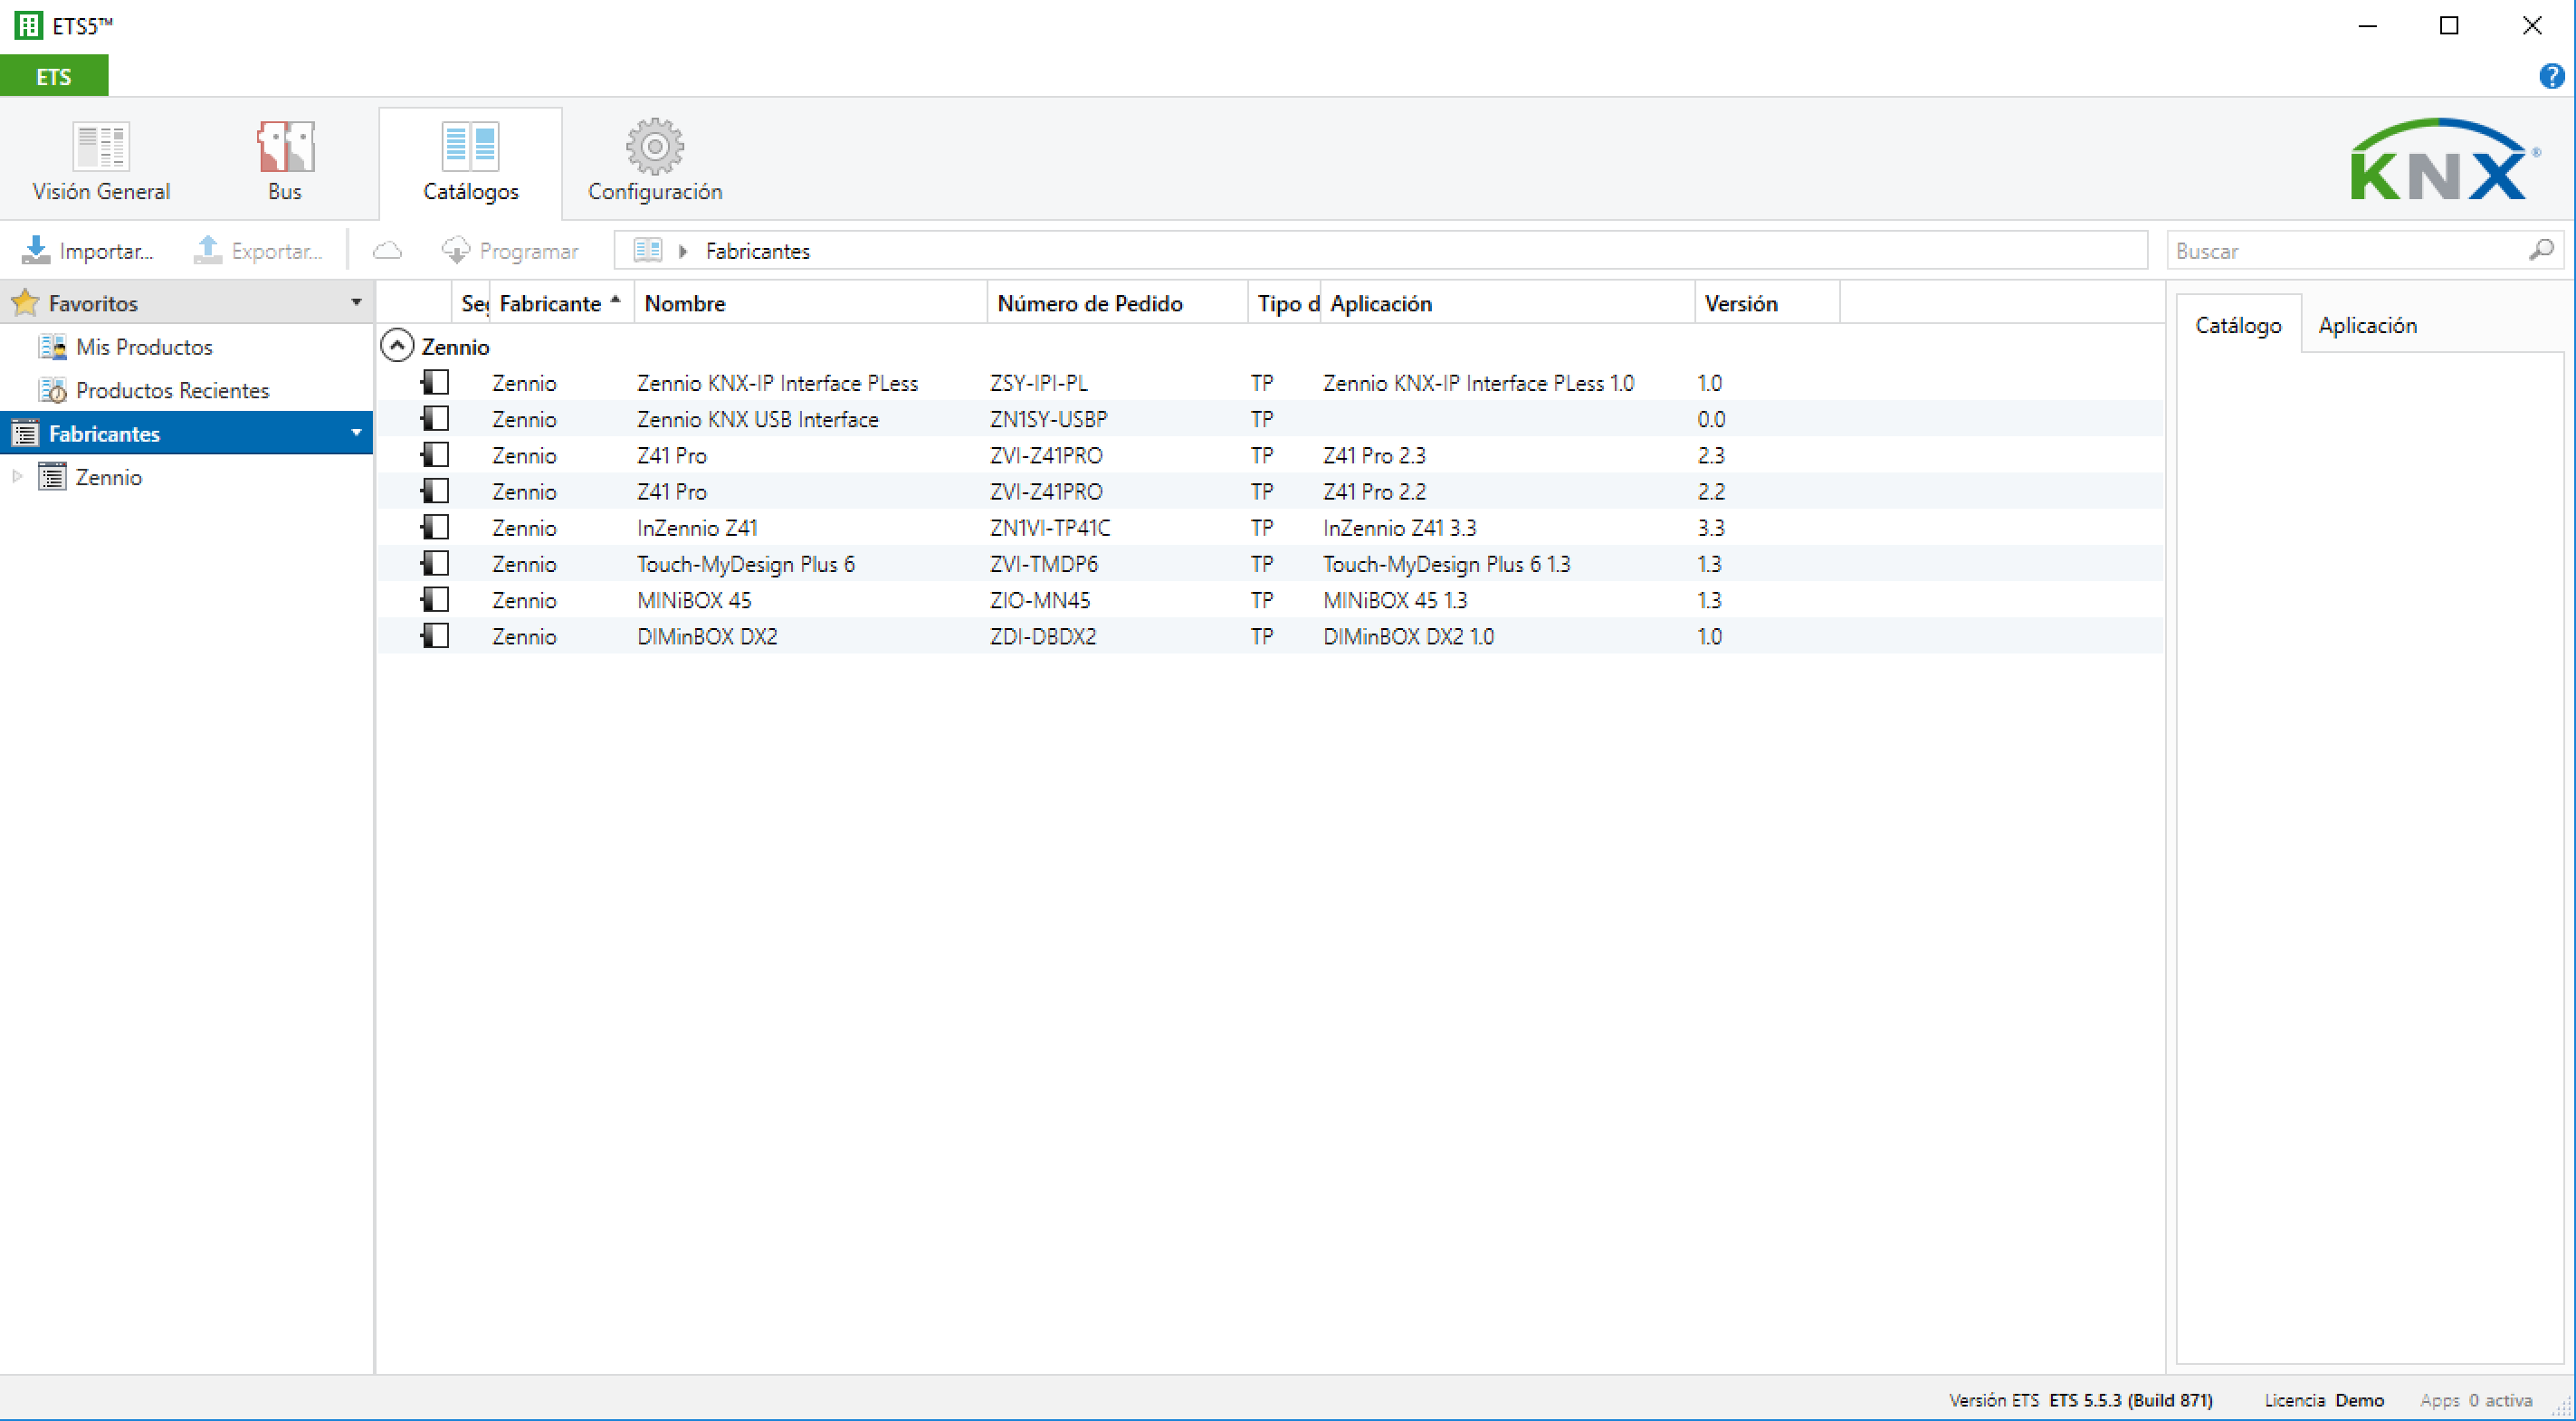
\includegraphics[width = 1.00\textwidth]{Imagenes/img1}
 		\captionof{figure}{\label{fig:IPN}Importando librerías.} 
	\end{center} 
\end{figure}

Ya esta el software preparado para comenzar a programar con los módulos del equipo de prácticas KNX en función de las necesidades que tenga cada situación como se irán describiendo en los siguientes puntos. \\


\section{Práctica 1. Regulación de luz.} 
La finalidad de esta primera práctica es la de realizar una funcionalidad que sea capaz de regular la intensidad luminosa de una lámpara led a través del módulo de botonera táctil. Para el desarrollo de esta primera situación se van a utilizar los módulos \textbf{DIMinBOX DX2} y \textbf{Touch-MyDesign Plus 6} del equipo KNX, por lo que los agregamos a nuestros dispositivos. El dispositivo \textbf{DIMinBOX DX2} se situará en el armario, mientras que el \textbf{Touch-MyDesign Plus 6} se colocará en el salón como se muestra en la siguiente figura. \\

\begin{figure}[H]
	\begin{center}
	 		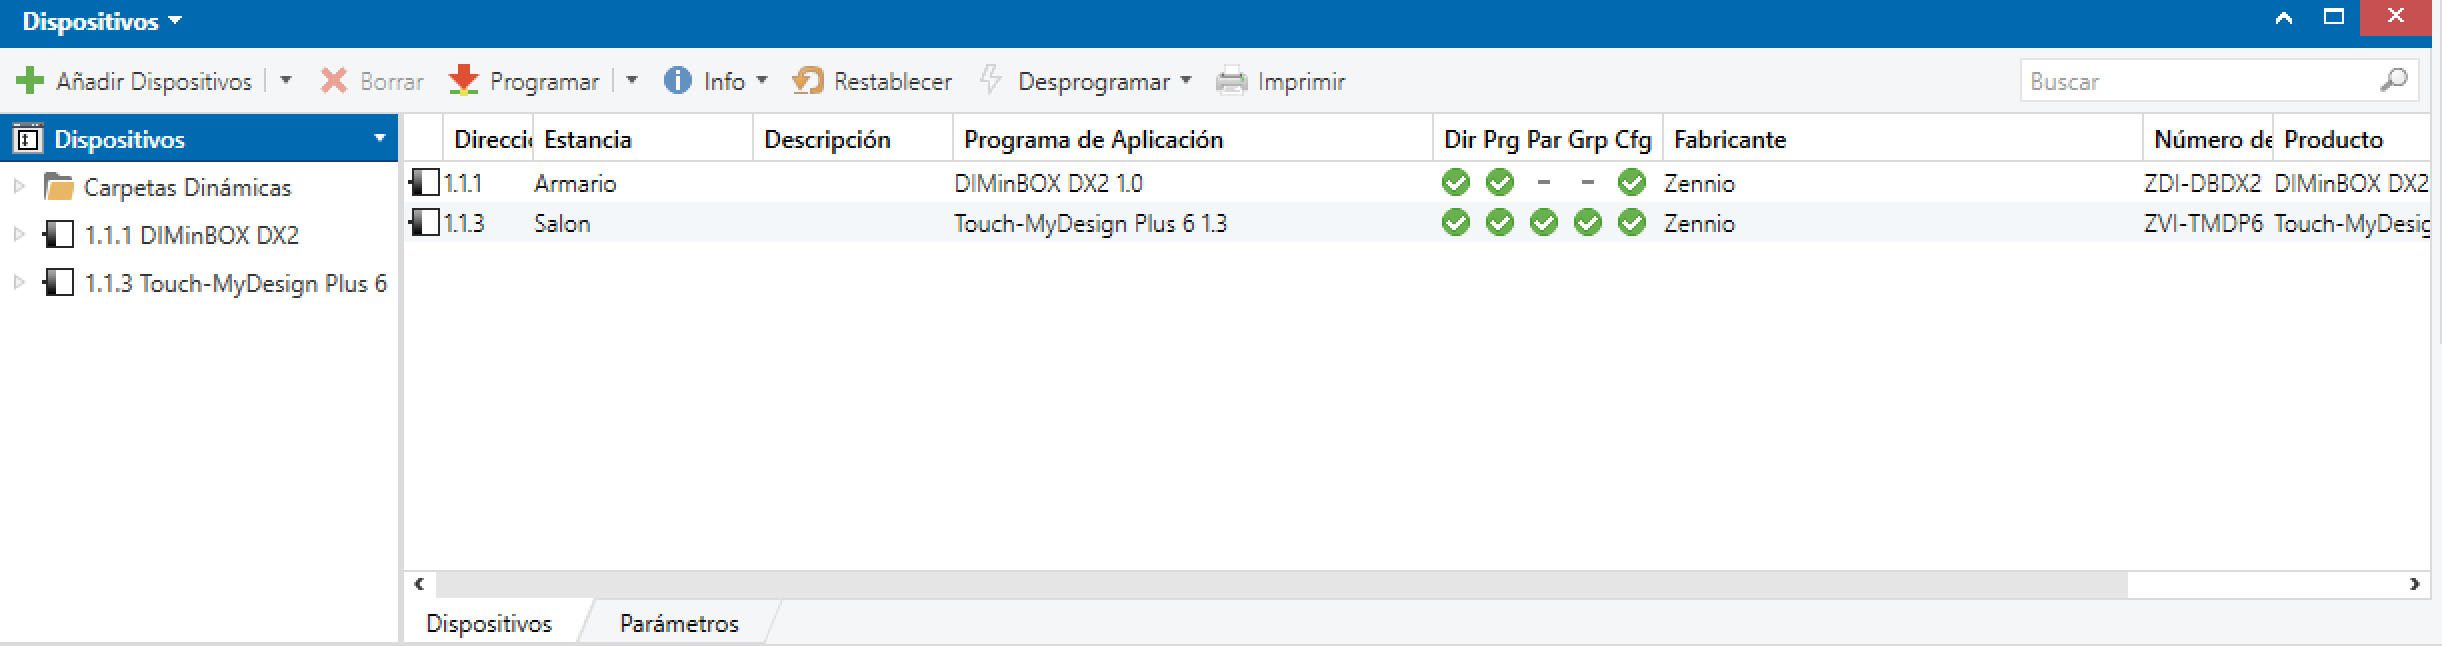
\includegraphics[width = 1.00\textwidth]{Imagenes/img2}
 		\captionof{figure}{\label{fig:IPN}Agregando dispositivos.} 
	\end{center} 
\end{figure}

Con los dispositivos agregados pasamos a configurar sus parámetros. El  \textbf{DIMinBOX DX2} dispone de dos salidas \textbf{C1} y \textbf{C2} que se encuentran conectadas a dos lámparas led de 220V, para nuesto supuesto vamos a utilizar las dos para controlar la regulación de la luz. \\

\begin{figure}[H]
	\begin{center}
	 		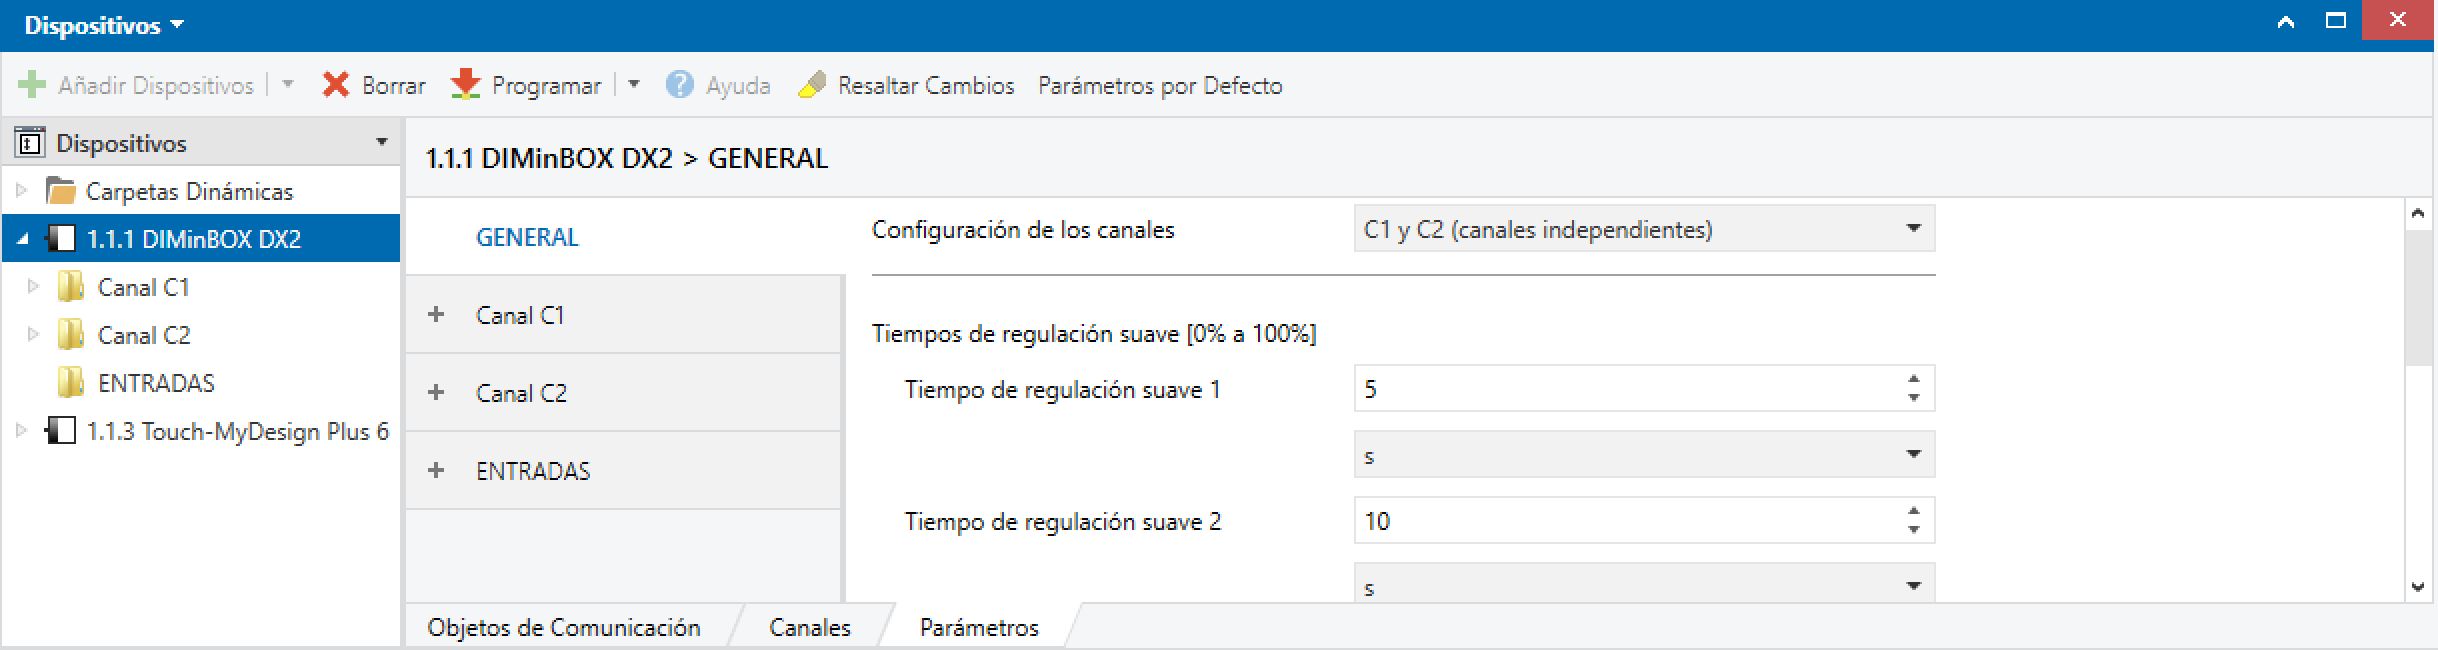
\includegraphics[width = 1.00\textwidth]{Imagenes/img3}
 		\captionof{figure}{\label{fig:IPN}Configurando parámetros del \textbf{DIMinBOX DX2}.} 
	\end{center} 
\end{figure}

Una vez que se han configurado los parámetros de dicho dispositivo, podemos ver los objetos de comunicación de los que dispone cada uno de las dos entradas del citado módulo. \\

\begin{figure}[H]
	\begin{center}
	 		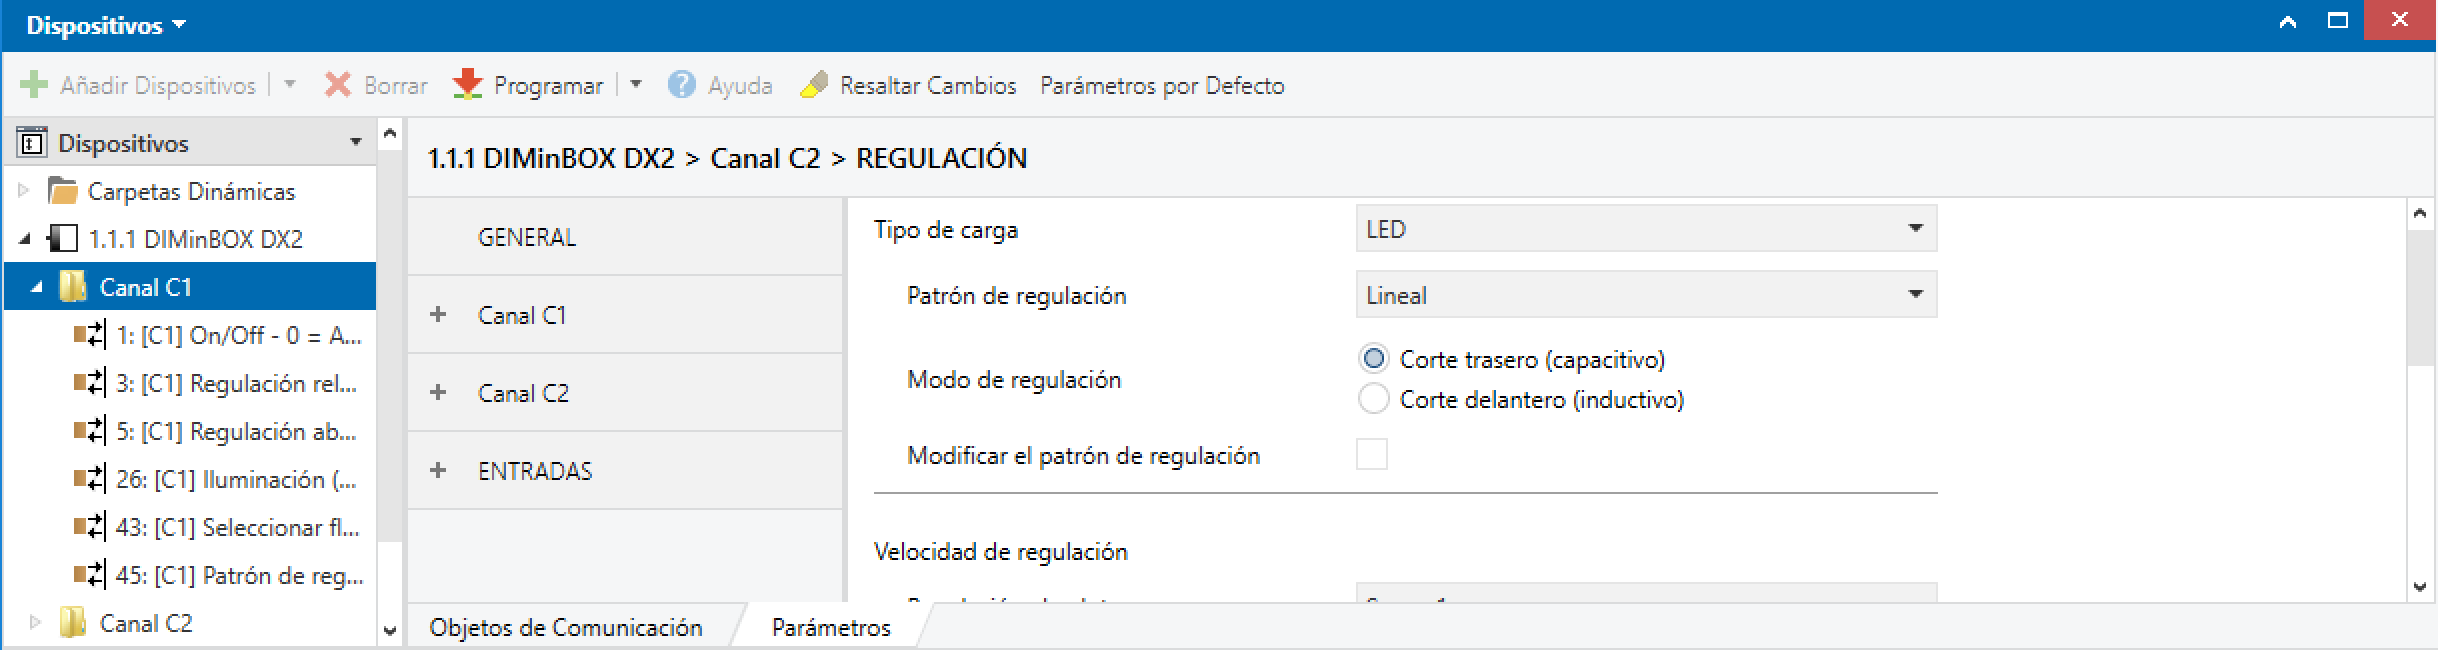
\includegraphics[width = 1.00\textwidth]{Imagenes/img4}
 		\captionof{figure}{\label{fig:IPN}Objetos de comunicación para \textbf{C1}.} 
	\end{center} 
\end{figure}

\begin{figure}[H]
	\begin{center}
	 		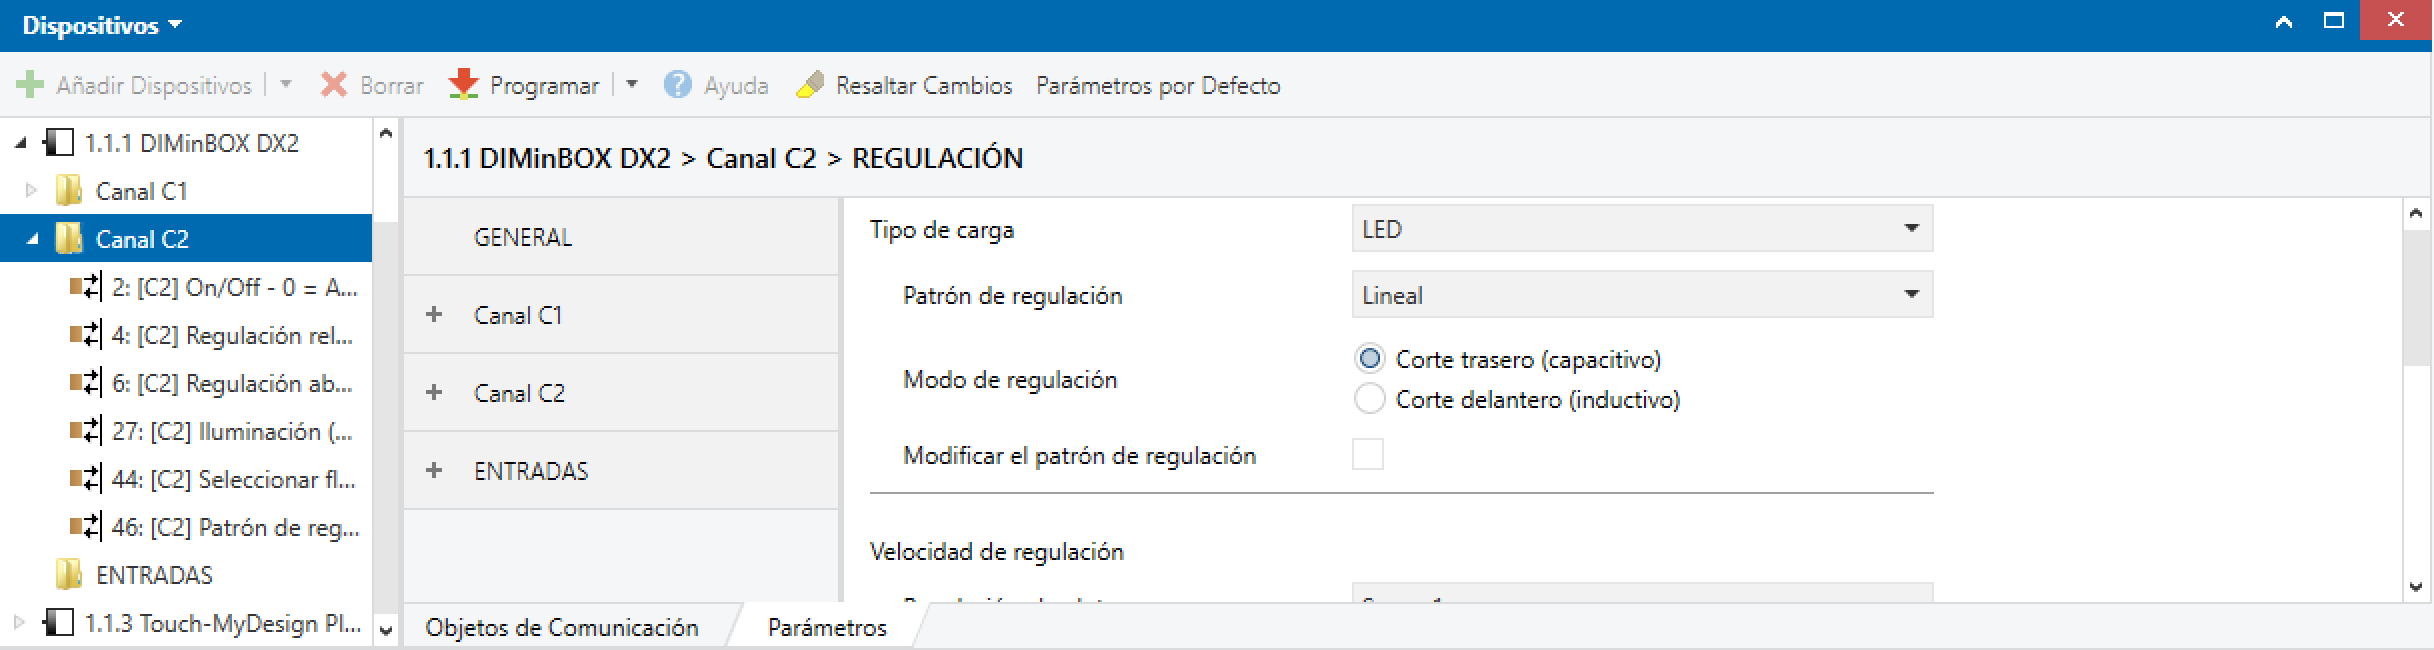
\includegraphics[width = 1.00\textwidth]{Imagenes/img5}
 		\captionof{figure}{\label{fig:IPN}Objetos de comunicación para \textbf{C2}.} 
	\end{center} 
\end{figure}

Ahora es el turno de configurar los parámetros del módulo \textbf{Touch-MyDesign Plus 6}. Para este dispositivo configuraremos uno de los pulsadores principales (\textbf{A1}) al cual le daremos una función de ``binario'' junto a una acción de ``conmutador''. En cuanto a la pareja B de este pulsador principal le estableceremos una función de ``control de regulador'' así como un paso de regulación del 25\%. \\

\begin{figure}[H]
	\begin{center}
	 		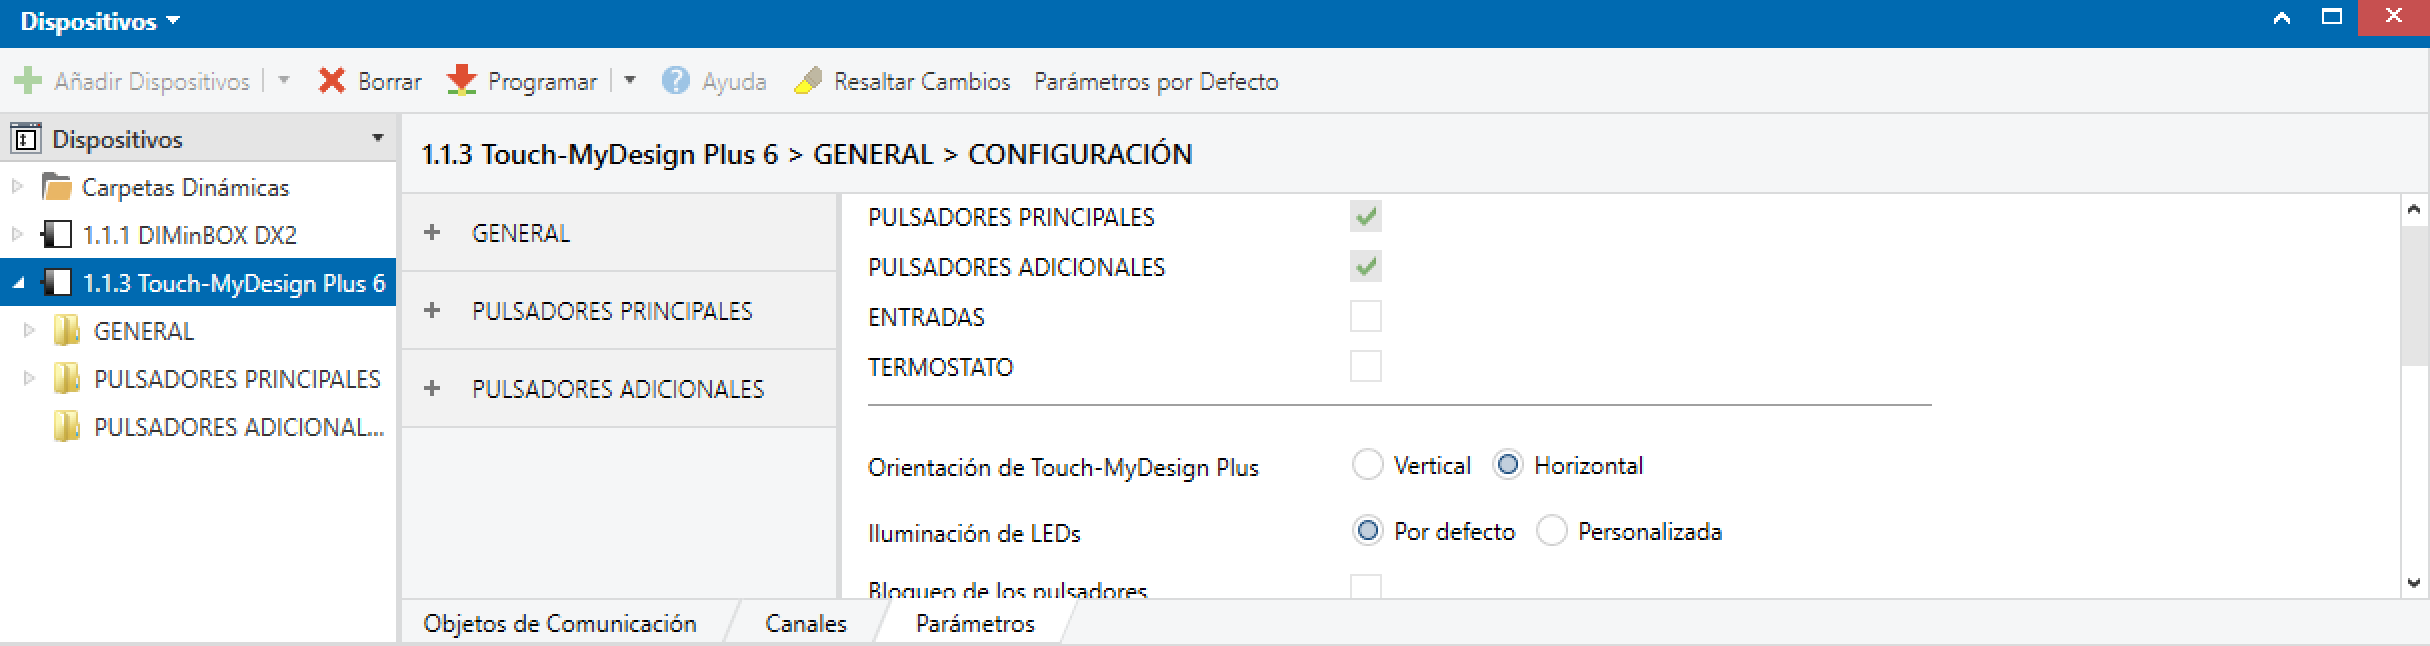
\includegraphics[width = 1.00\textwidth]{Imagenes/img6}
 		\captionof{figure}{\label{fig:IPN}Configurando parámetros del \textbf{Touch-MyDesign Plus 6} (I).} 
	\end{center} 
\end{figure}

\begin{figure}[H]
	\begin{center}
	 		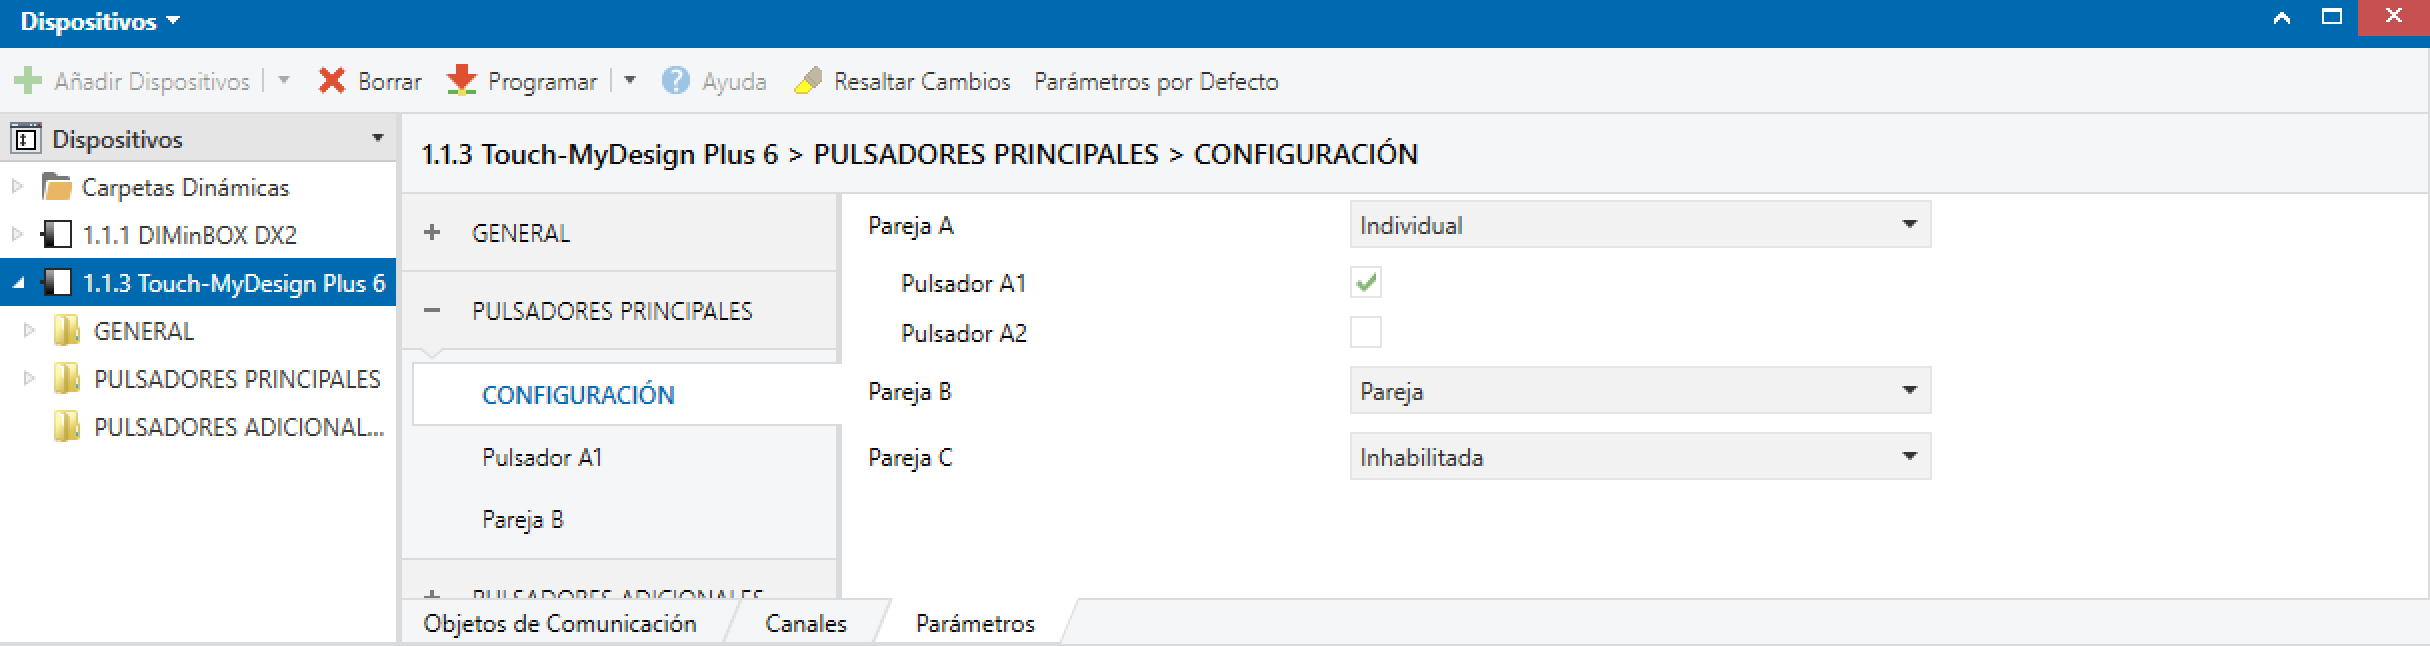
\includegraphics[width = 1.00\textwidth]{Imagenes/img7}
 		\captionof{figure}{\label{fig:IPN}Configurando parámetros del \textbf{Touch-MyDesign Plus 6} (II).} 
	\end{center} 
\end{figure}

\begin{figure}[H]
	\begin{center}
	 		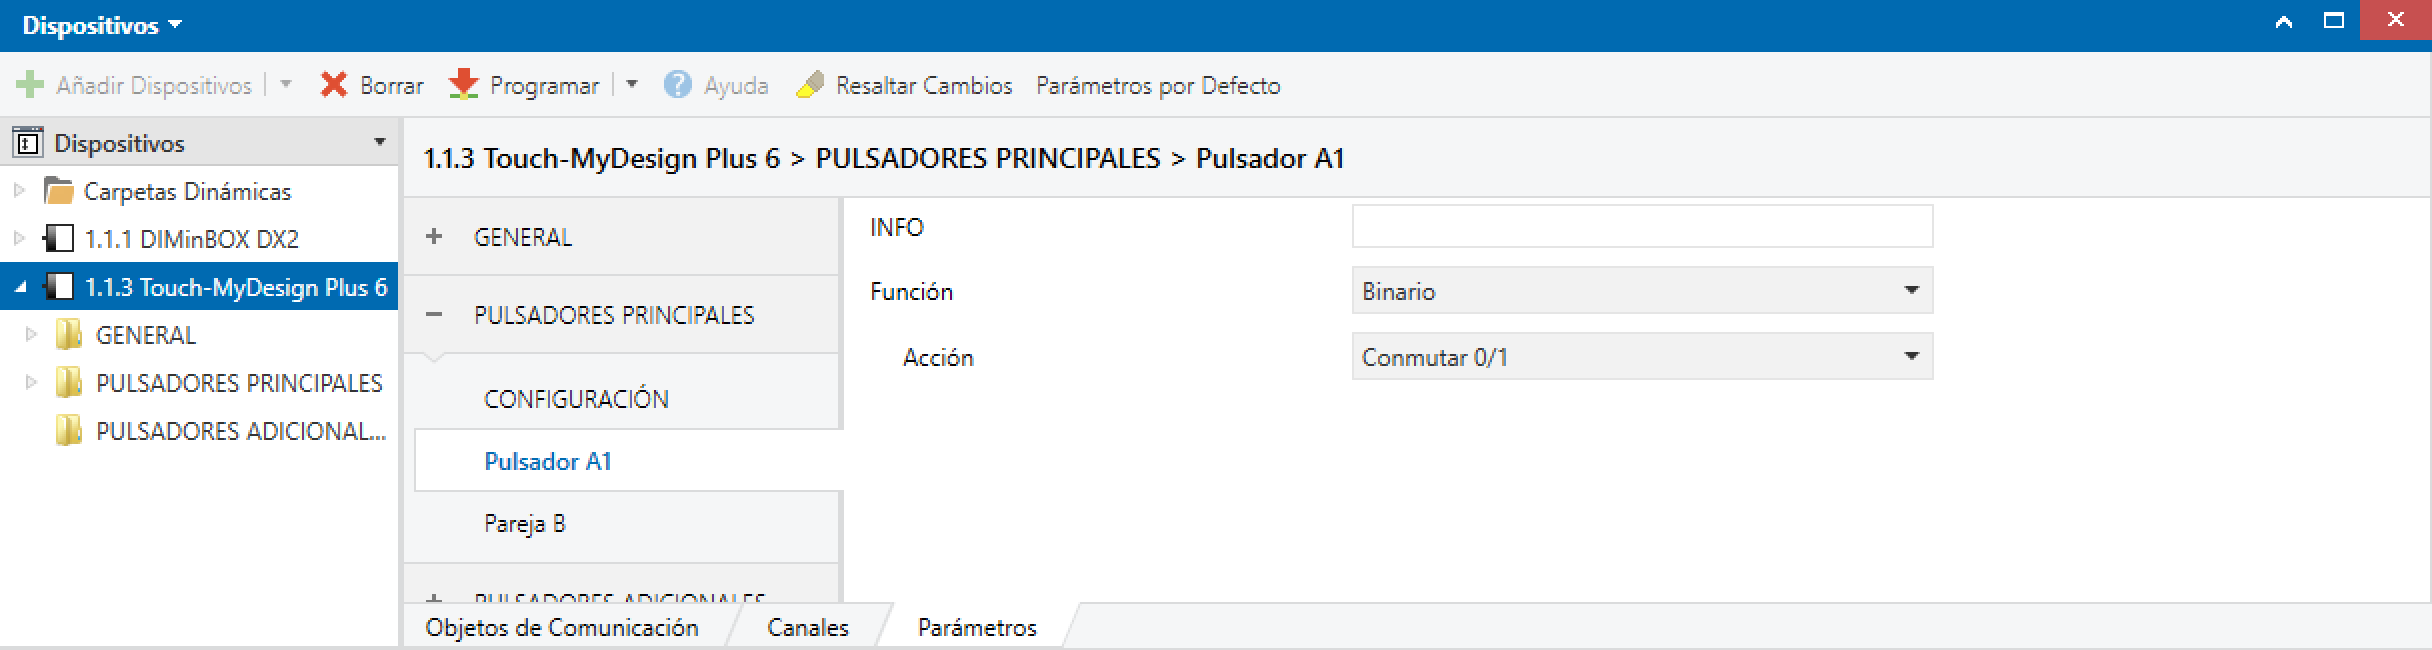
\includegraphics[width = 1.00\textwidth]{Imagenes/img8}
 		\captionof{figure}{\label{fig:IPN}Configurando parámetros del \textbf{Touch-MyDesign Plus 6} (III).} 
	\end{center} 
\end{figure}

\begin{figure}[H]
	\begin{center}
	 		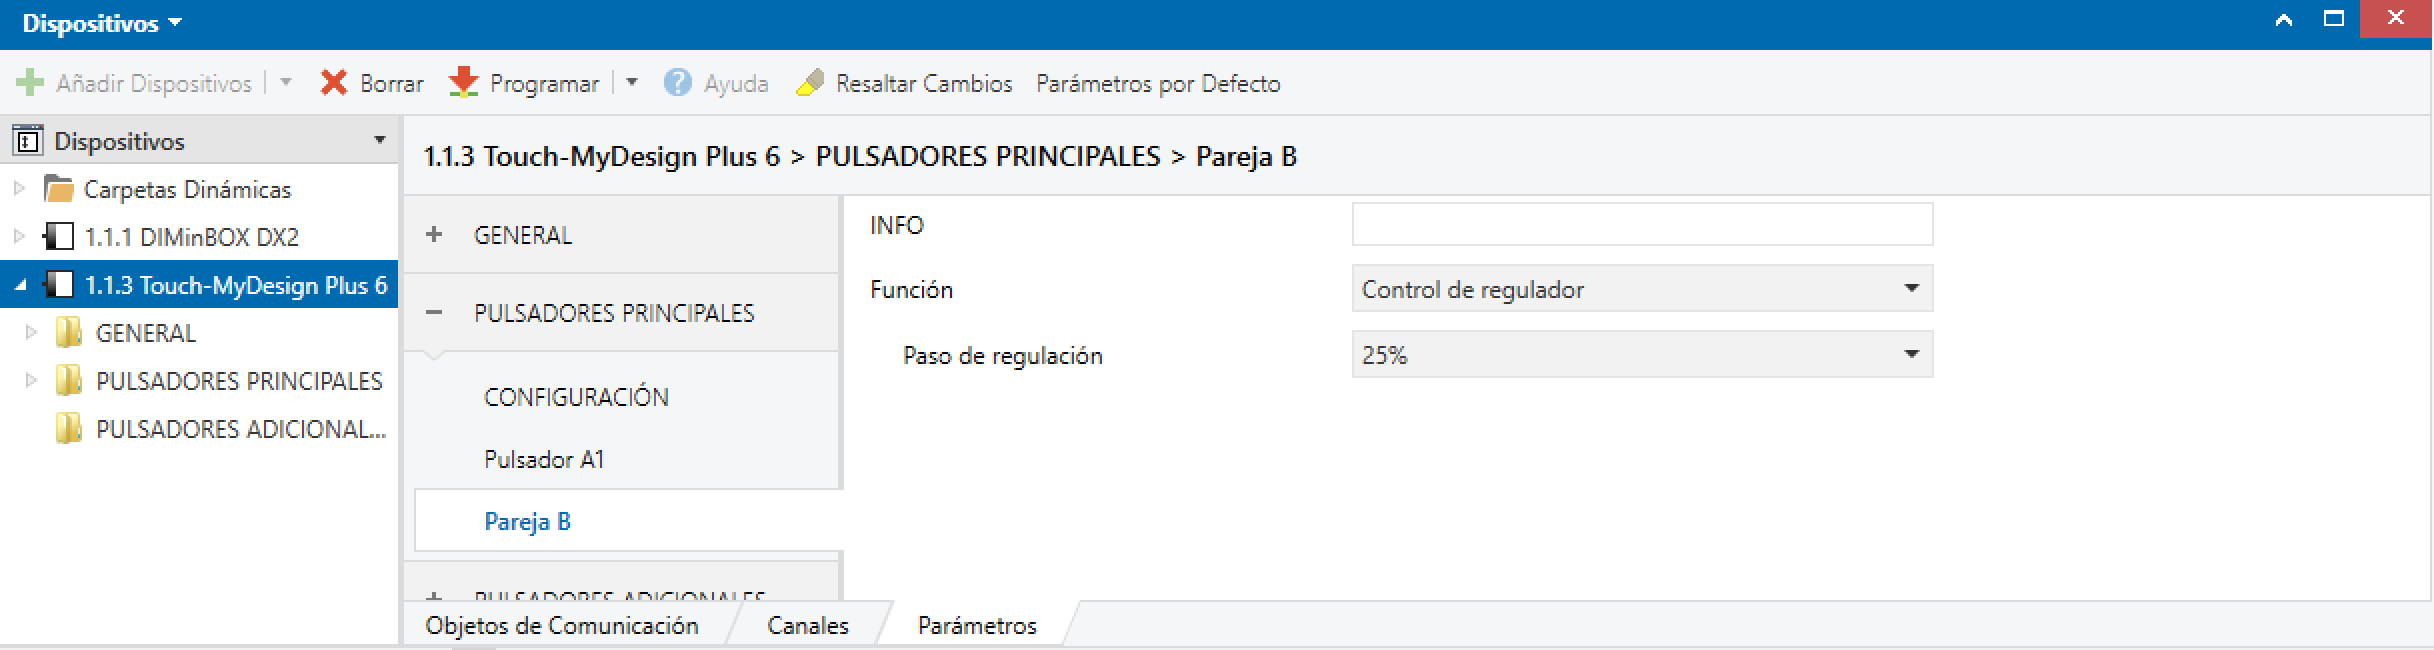
\includegraphics[width = 1.00\textwidth]{Imagenes/img9}
 		\captionof{figure}{\label{fig:IPN}Configurando parámetros del \textbf{Touch-MyDesign Plus 6} (IV).} 
	\end{center} 
\end{figure}

Pasamos ahora a definir las direcciones de grupo donde incluiremos los objetos de comunicación necesarios. Disponemos del grupo principal llamado \textbf{iluminación}, el cual contiene al grupo intermedio \textbf{Salón} del que a su vez cuelgan las direcciones de grupo \textbf{OnOff\_Luz\_Techo} y \textbf{Regulación}. \\

\begin{figure}[H]
	\begin{center}
	 		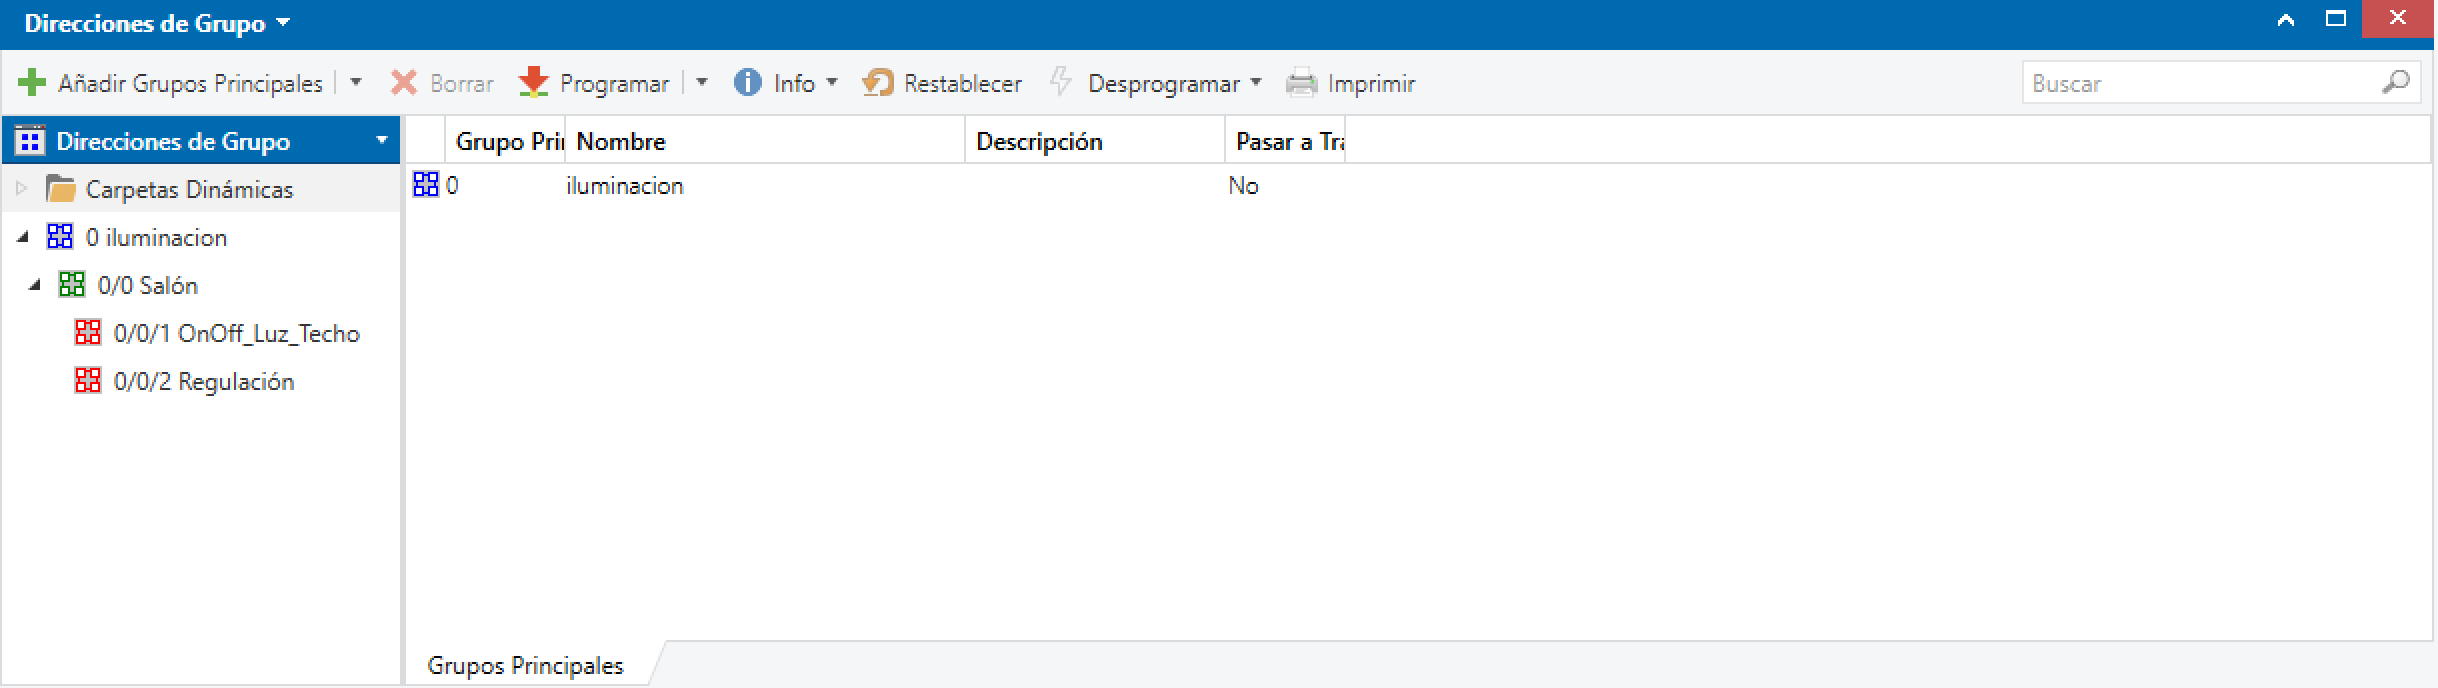
\includegraphics[width = 1.00\textwidth]{Imagenes/img10}
 		\captionof{figure}{\label{fig:IPN}Estableciendo las direcciones de grupo.} 
	\end{center} 
\end{figure}

A la dirección de grupo \textbf{OnOff\_Luz\_Techo} le añadiremos los objetos de comunicación ``On/Off'' del dispositivo \textbf{DIMinBOX DX2} de la salida \textbf{C1} y el objeto de comunicación ``Control binario'' del pulsador principal \textbf{A1} perteneciente al dispositivo  \textbf{Touch-MyDesign Plus 6}. \\

\begin{figure}[H]
	\begin{center}
	 		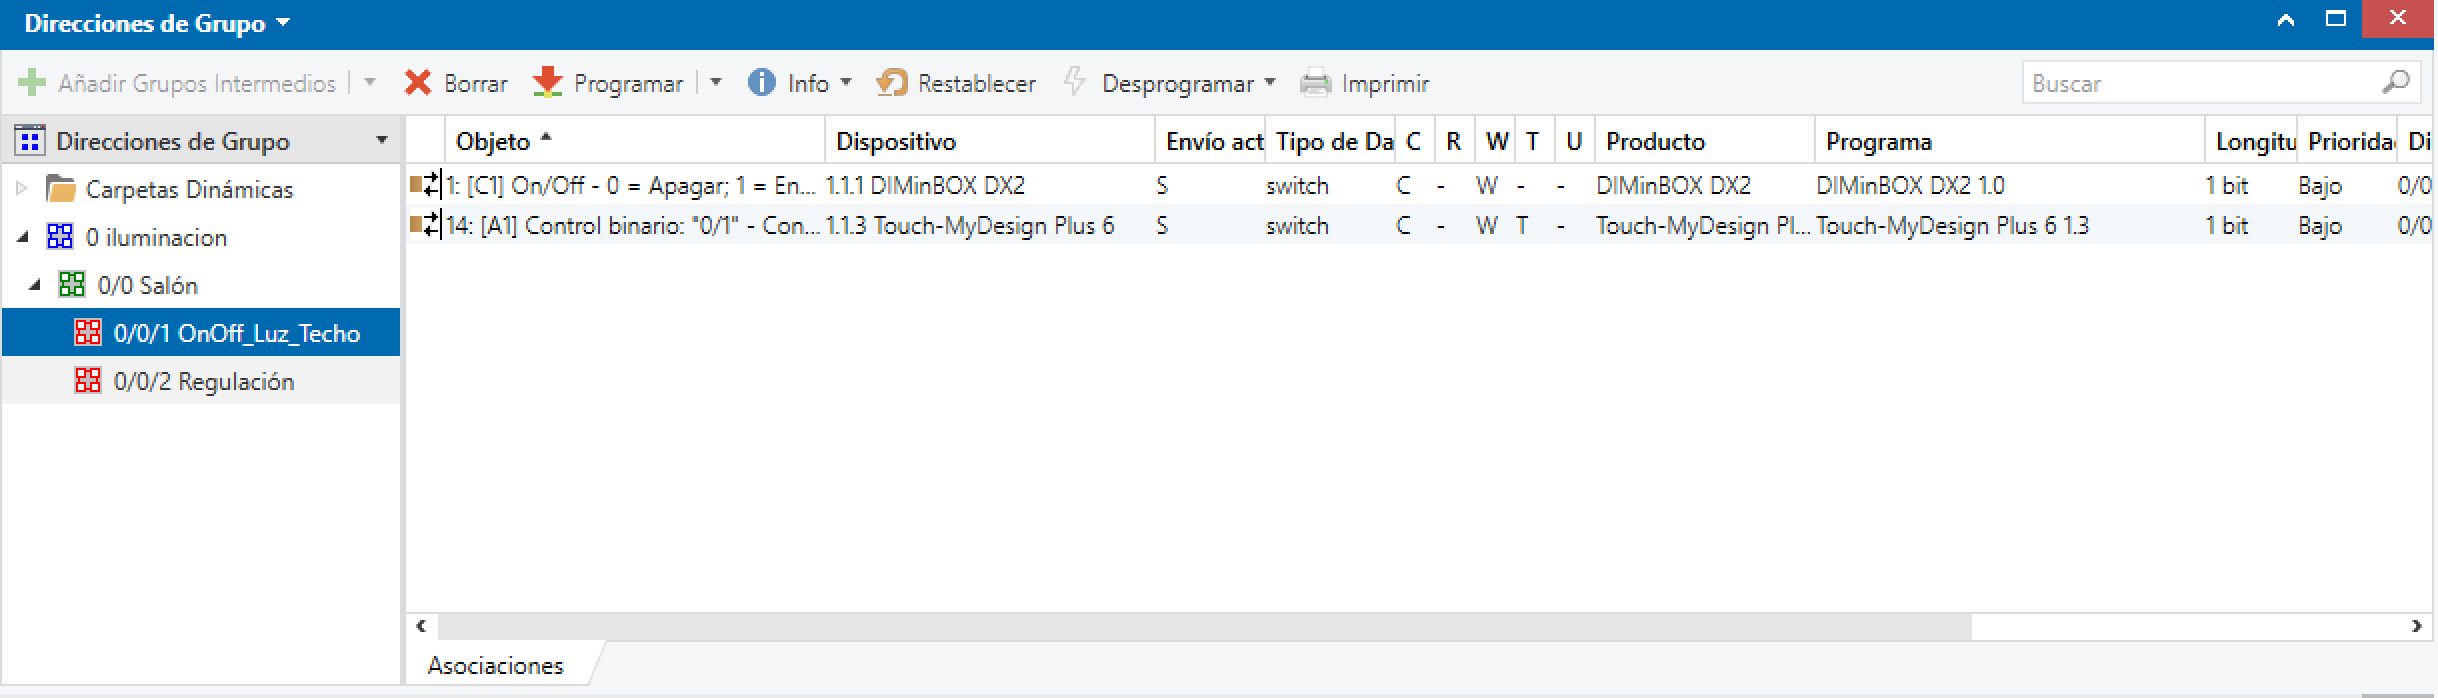
\includegraphics[width = 1.00\textwidth]{Imagenes/img11}
 		\captionof{figure}{\label{fig:IPN}Añadiendo objetos de comunicación a la dirección de grupo \textbf{OnOff\_Luz\_Techo}.} 
	\end{center} 
\end{figure}

\begin{figure}[H]
	\begin{center}
	 		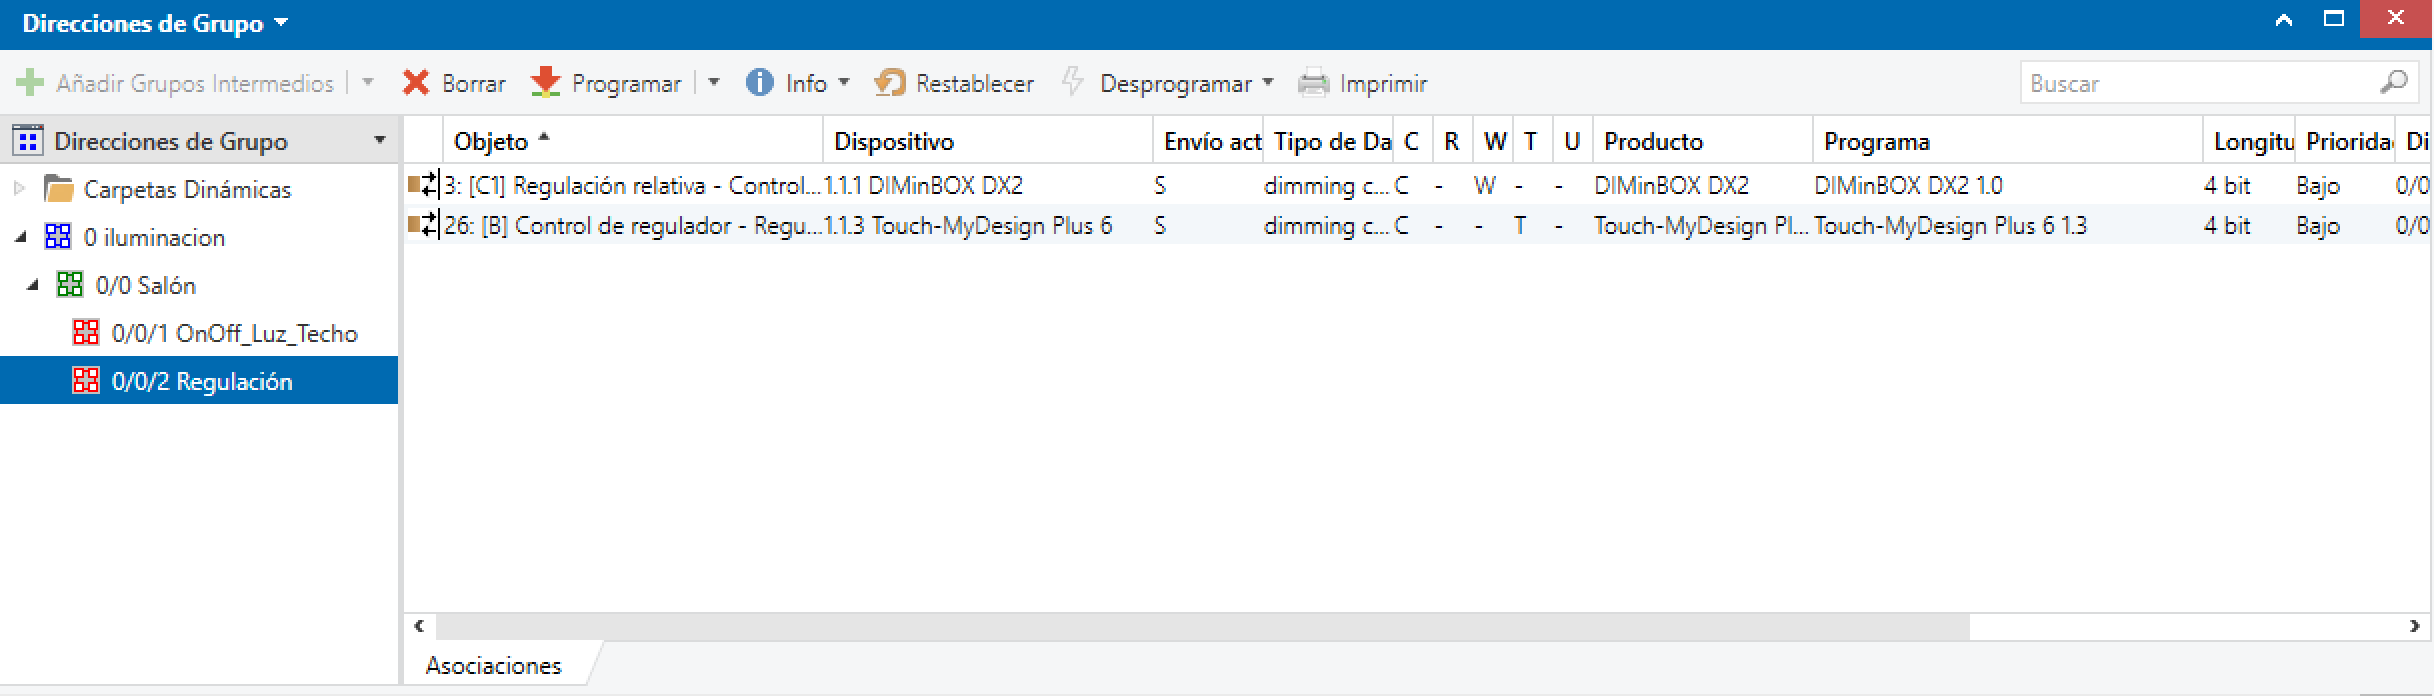
\includegraphics[width = 1.00\textwidth]{Imagenes/img12}
 		\captionof{figure}{\label{fig:IPN}Añadiendo objetos de comunicación a la dirección de grupo \textbf{Touch-MyDesign Plus 6}.} 
	\end{center} 
\end{figure}

Terminada esta configuración, el sitema queda totalmente configurado para ser programado y lanzado en el entorno de pruebas KNX. \\


\end{document}
